%%%%%%%%%%%%%%%%%%%%%%%%%%%%%%%%%%%%%%%%%%%%%%%%%%%%%%%%%%%%%%%%%%%%%%%%%%%%%%%%
%2345678901234567890123456789012345678901234567890123456789012345678901234567890
%        1         2         3         4         5         6         7         8

\documentclass[letterpaper, 10 pt, conference]{ieeeconf}  % Comment this line out if you need a4paper

%\documentclass[a4paper, 10pt, conference]{ieeeconf}      % Use this line for a4 paper

\IEEEoverridecommandlockouts                              % This command is only needed if 
                                                          % you want to use the \thanks command

\overrideIEEEmargins                                      % Needed to meet printer requirements.

%In case you encounter the following error:
%Error 1010 The PDF file may be corrupt (unable to open PDF file) OR
%Error 1000 An error occurred while parsing a contents stream. Unable to analyze the PDF file.
%This is a known problem with pdfLaTeX conversion filter. The file cannot be opened with acrobat reader
%Please use one of the alternatives below to circumvent this error by uncommenting one or the other
%\pdfobjcompresslevel=0
%\pdfminorversion=4

% See the \addtolength command later in the file to balance the column lengths
% on the last page of the document

% The following packages can be found on http:\\www.ctan.org
\usepackage{graphics} % for pdf, bitmapped graphics files
\usepackage{epsfig} % for postscript graphics files
%\usepackage{mathptmx} % assumes new font selection scheme installed
%\usepackage{times} % assumes new font selection scheme installed
%\usepackage{amsmath} % assumes amsmath package installed
%\usepackage{amssymb}  % assumes amsmath package installed
\usepackage{algorithm}
\usepackage{algpseudocode}

\title{\LARGE \bf
Explaining and Interpreting Model Predictions for Short Answer Grading*
}


\author{Ravikiran Bhat, Deebul Nair$^{1}$ and Paul G. Pl{\"o}ger$^{2}$% <-this % stops a space
%\thanks{*This work was not supported by any organization}% <-this % stops a space
\thanks{$^{1}$Deebul Nair is with Faculty of Computer Science,
        University of Applied Sciences Bonn-Rhein-Sieg, Sankt Augustin, Germany7/
        {\tt\small deebul-sivarajan.nair@h-brs.de}}%
\thanks{$^{2}$Bernard D. Researcheris is the Vicedean of the Department of Computer Science, Autonomous Systems, University of Applied Sciences Bonn-Rhein-Sieg, Sankt Augustin, Germany
        {\tt\small paul.ploeger@h-brs.de}}%
}


\begin{document}



\maketitle
\thispagestyle{empty}
\pagestyle{empty}


%%%%%%%%%%%%%%%%%%%%%%%%%%%%%%%%%%%%%%%%%%%%%%%%%%%%%%%%%%%%%%%%%%%%%%%%%%%%%%%%
\begin{abstract}

This work focuses on associating a reasoning for automated scores for short answers type questions as a means of rationalizing the predicted score to the human graders. Observations resulting from the pre-investigations conducted on two state-of-the-art model-agnostic interpretation techniques, namely, LIME and SHAP serves as the inspiration in the development of our solution. In our work, by relying on a simple BOW model supported by active learning, we develop an algorithm and a grading assisting tool that supports human graders with automated grading together with highlighted features acting as supporting explanations to enable the human graders to interpret the cause of the suggested grades. 

\end{abstract}


%%%%%%%%%%%%%%%%%%%%%%%%%%%%%%%%%%%%%%%%%%%%%%%%%%%%%%%%%%%%%%%%%%%%%%%%%%%%%%%%
\section{INTRODUCTION}

....

\section{RELATED WORK}
The methodology presented in [1] is the closest related work to our research and is also one of the most promising works in the field of model interpretation and explanations. The \textit{LIME} (Local interpretable model-agnostic explanations) method presented in this paper approximates a black-box model locally in the neighborhood of a specific prediction, i.e, it fits local, interpretable models that can explain predictions for a specific instance of \textit{any} classifier. The novelty behind LIME is that the model agnostic explanations of LIME are produced in the form of color coded features in the text that are easily understood even by human users with no underlying knowledge of the working of the model used to classify the predictions. These explanations are useful in many scenarios that require promoting trust in a prediction and is helpful in determining whether a classifier should be trusted or not. Similarly belonging to the class of model-agnnostic model interpretation methods is the SHAP (SHapley Additive exPlanations) framework presented by Lundberg et. al in [2] that leverages the concept of Shapley values explanations from cooperative game theory. The SHAP method presented in the paper assigns each feature an importance value and use them to explain predictions. Since method of computing the SHAP values involves the exhaustive approach of computing the ``average marginal contribution of a feature value over all possible coalitions"[3], it theoretically guarantees the properties of accuracy and consistency.

\section{PRE-INVESTIGATIONS}

This section describes a series of investigative experiments which are responsible for determining the main areas of focus in our solution design. Two of the existing model interpretation techniques from literature, namely LIME and SHAP were the main focus of the experiments. All experiments are carried out via a supervised learning process with 65\% of the data used as the training set and the rest for testing. We use a Bag of Words (BOW) approach as the basis for extracting ngrams and use them as predictors for the scores and Naive Bayes classifier was used as the learning model to classify the discrete features. The the grading is treated as a binary classification task with each answer graded as correct or incorrect. The observations from the experiments were used to narrow down the shortcomings of the two model interpretation techniques that we attempt to address in our future solution design. The experiments in this section therefore serve as a benchmark that heavily influences the direction of our approach discussed in the next section.

\subsection{Datasets} 

All experiments in this section were conducted on datasets from two sources:
\begin{enumerate}
\item \textbf{Mohler's Dataset}\\
The dataset consists of a set of questions taken from assignments given out for the Data Structure course at the University of North Texas \cite{mohler2011learning}. The answers were collected from a class of 31 undergraduate students via an online learning assignment. The dataset was created by working on student answers for 80 different questions and a total of 2273 answers. The answers were scored independently by two human graders on scale ranging from 0 (completely incorrect) to 5 (perfect answer). In our pre investigations, student scores above 3 were labeled as `Correct' and those graded 3 or lower were labeled as `Incorrect'. 
\item \textbf{Neural Network Dataset}\\
This dataset consists of 17 questions administered as part of the Neural Networks course examination at the University of applied sciences Bonn-Rhein-Sieg. The answers were collected from a class of 39 students from an online examination conducted using Jupyter Notebooks. The dataset was created by using the student answers for the first 17 questions which required mandatory answers. The answers were scored on an integer scale as either 0(completely incorrect), 1 (partially correct) or 2 (perfect answer). In our pre investigations, student scores below 2 points were labelled as `Incorrect' and those with 2 points were labelled as `Correct'.
\end{enumerate}
A total of 14 questions selected from both datasets acted as case studies in our experiments. The questions selected included those which required answers in a few words (i.e not exceeding 4-5 words), in one or two sentences, and those where answers were longer than two to three sentences. A sub goal of the investigations in this section was to narrow down the attributes of the questions for which the applied interpretability techniques gives the best results matching human expectations.
\subsection{Data Preprocessing}
A separate model is learned after extracting features from the answers to each question. Before extracting features and learning a model, the answers from the two datasets are subject to preprocessing using NLP techniques:
\begin{itemize}
\item The model answers and student answers were tokenized into words and all words were converted into lowercase form.
\item The segmented text obtained from the previous step was then subjected to stopword removal.
\item Lemmatization was performed in order to obtain the base / dictionary form of a word after removing the inflectional endings in each word.
\end{itemize}

\subsection{Benchmarking Experiments}
Two experiments are conducted to check the differences in the degree of understanding gained from the explanations given by LIME and SHAP.
\begin{enumerate}
\item \textit{Experiment 1}:\\
In this experiment, LIME is applied on the unseen test instances  to get an explanation that is locally faithful to the classifier. This experiment is divided into 2 parts. In the first part, we experiment with two feature extractors, namely `CountVectorizer' which gives a a sparse matrix representation of the token counts from the student answers, and the TfidfVectorizer that gives a normailzed score for each of the word occurance count. The goal of the first part of the experiment is determine the best feature extractor by observing the influence  on the final LIME explanation. In the second part of the experiment, we focus on the explanation obtained for every test instance for every case study to determine the degree of understanding gained for different answers, and also narrow down the limitations in the explanations that needs to be addressed.
\item \textit{Experiment 2}:\\
In this experiment, we apply Shapley value explanations as the model-agnostic interpretation technique for our predicted scores. The SHAP (SHapley Additive exPlanations) library
introduced by Lundberg et al.[2] is used to visualize a global overview of the impact of the top k features on the model output. The goal of this experiment is to analyze the global interpretation obtained from SHAP and contrast it with the locally faithful explanations generated by LIME.
\end{enumerate}
\subsection{Benchmarking Experiments' Results and Analysis}
\textit{Experiment 1:}\\
Results of experiment 1 showed that, contrary to expectations, performance in terms of the final accuracy as well as the explanations from LIME were identical for both CountVectorizer and TfidfVectorizer. Observing the predictions and explanations on unseen data, it was seen that while very few instances showed some minor differences in the highlighting of unigrams, these differences did not have any noticeable impact on the interpretation gained by the end user. Some other general observations on the LIME explanations summarized below:
\begin{itemize}
\item The shorter the answer length, the closer the highlighted unigrams was to human expectations. 
\item Lower model accuracies consequently ended up affecting not only the predicted scores, but the resulting LIME highlighted explanations also tended to being more unacceptable by humans.
\item Larger answers and higher linguistic diversity in the student responses resulted in explanations that were inconceivable due to LIME's limitations in highlighting only unigrams in the text.
\end{itemize}
\textit{Experiment 2:}\\
We rely on the SHAP's summary plot to get a display of the top 20 globally important features affecting the model output for every answer in the test set to a given question. An example summary plot for the class ``Correct" showing the SHAP value for the most important features identified from among the test samples to the question: \textit{``What is the role of prototype program in problem solving?"} is shown in Figure \ref{fig:shap1} that has the following model answer in the dataset: \textit{``To simulate the behaviour of portions of desired software product"}. 
\begin{figure}[H]
\framebox{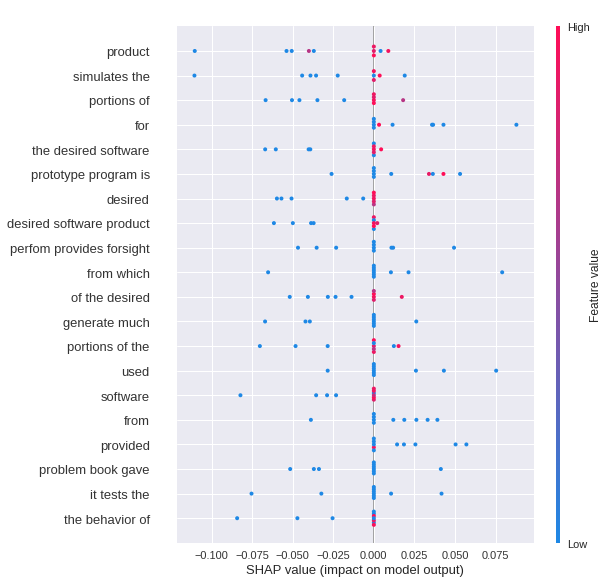
\includegraphics[width=0.48\textwidth, height=0.5\textwidth]{images/shap/all_features_0_nb.png}}
\caption{An example SHAP summary plot of top 20 features for the class ``Correct".}
\label{fig:shap1}
\end{figure}
Each dot in the plot represents one instance from the test set. The plot reveals that low values (i.e, the samples highlighted in blue) of features such as \textit{``simulates the"}, \textit{``portions of"}, \textit{``desired"} , \textit{``software"}, etc for samples (low here indicating the absence of said feature) will have negative influence on model output. This indicates that these features are important for a student answer to be classified as \textit{``Correct"}. Presence of these features in any sample (highlighted in red) will not influence the classification of the answer as \textit{``Correct"} in a negative way. This is an example of a case where a human's intuition of the features that are the most important predictors towards a particular class matches closely with the explanation displayed by the summary plot. After observing the summary plots for all the questions selected as our case studies, we come to the following conclusions on the global explanation from SHAP's summary plots:
\begin{itemize}
\item Questions with shorter answers(i.e, where length of answers was limited to maximum of one sentence) gave the best results in terms of the top features identified matching human expectations.
\item For questoins with longer answers and cases where there was a great amount of linguistic diversity between student answers, the features identified and/or the impacts shown on the model outputs in the plots were redundant and unconvincing. In such cases the global explanations given by the summary plots played no useful role, and great amount of effort from the user was needed to interpret the explanations.
\end{itemize}
Global interpretation such as the one described in the third experiment is useful in understanding and getting a sense of the magnitude and direction of influence of each feature on the prediction. Although SHAP’s strength lies in providing a globally consistent and accurate explanations by using an exhaustive approach of considering predictions for all possible coalitions for each feature, compared to LIME which is fast and where explanations are obtained instantaneously, computing the Shapley values for the features takes time in the order of 5-10 minutes. On the other hand, while LIME does not have the accuracy and consistency properties of Shapley values, LIME's output provided a more ``human friendly" explanation, and felt a more preferable choice when explaining the cause of predictions to end users.
\subsection{Quantitative Benchmarking}
In this section, we attempt to quantitatively evaluate and measure the level of interpretation gained from LIME's local explanations and SHAP's global explanation. However, with no clear consensus or ground truth available to compare different interpretations techniques, we developed a strategy whereby an initial qualitative assessment of the explanations was done followed by a mapping to a value within a fixed range  to get an idea of how the two interpretation techniques measure against each other in their explanations for the different cases studies. This evaluation is carried out by the experimenter with concrete procedure being as follows:
\begin{itemize}
\item When using LIME to get explanations for a student answer, we assign a score on a 3 point Likert scale(i.e, from 1-3) to indicate the degree to which the explanation is acceptable( 1 being the lowest, and 3 being the highest score indicating that a human user completely agrees with the explanation.
\item In case of SHAP's global explanations from summary plots, we score the explanation based on how accurately we feel the features and their impacts have been captured in the visualization. In case of SHAP, a 3-point Likert scale range was insufficient to capture the level of interpretability, understanding and satisfaction from the explanation obtained by the user, and thus used a wider 5-point scale was used.
\end{itemize}
Ordinal data captured using the above method was then mapped to a single value in the range [0,1] for each question acting as the case study which served as our interpretation level for comparsion. The mapping was done as follows:
\begin{itemize}
\item In case of LIME, after giving an ordinal score for each instance of student answer for a question, we compute the ratio of the occurrences for each type of ordinal score.
\item We rely on  SciPy library’s interpolation function to perform the following mappings:
\begin{itemize}
\item Ratios computed for ordinal value \textbf{1} is mapped from [0, 1] $=>$ [0, 0.33] range.
\item Ratios computed for ordinal value \textbf{2} is mapped from [0, 1] $=>$ [0.34, 0.66] range.
\item Ratios computed for ordinal value \textbf{3} is mapped from [0, 1] $=>$ [0.67, 1] range. 
\end{itemize}
\item The mapping obtained for the ordinal value with the largest ratio in the data for a given question is taken to be the Interpretation Level (IL) for that In case we have a situation where more than one type of ordinal score has the same maximum ratio of occurrences (for e.g ordinal scores 1 and 2 both having a ratio 6 out of a total of 15 samples), in such a case we simply take the average of those ordinal scores, and the average value that lies between 1 and 3 is mapped to [0,1] range directly. 
\item In case of SHAP, the ordinal data was directly mapped to the [0, 1] range which corresponded to the Interpretation Level (IL) for SHAP for that question.
\end{itemize}
The Figure \ref{fig:comparison1} shows the comparison of the interpretation levels for every question used as case study from the Mohler's dataset.
\begin{figure}[H]
\framebox{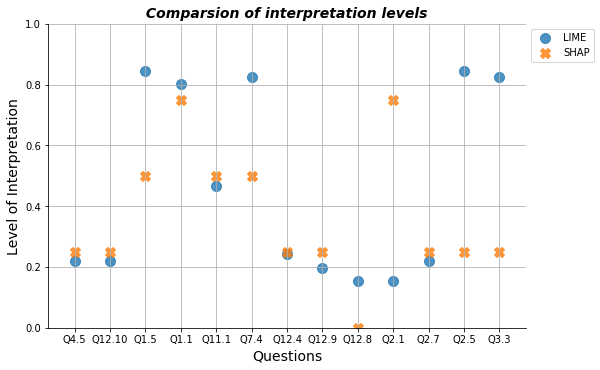
\includegraphics[width=0.48\textwidth, height=0.4\textwidth]{images/all_categ.png}}
\caption{Quantitative Interpretation Level comparison of LIME and SHAP for different questions.}
\label{fig:comparison1}
\end{figure}
As observed from the figure, in majority of the cases LIME results in either a comparable or higher interpretation level from its explanations. This stems from the reason that LIME's explanation being more human friendly and are more geared towards explaining the predictions to laypersons when compared to SHAP.
\section{PROPOSED SOLUTION}

The algorithm developed in this work was aimed with end goal of predicting and presenting student textual responses such that a human end user's understanding of the relation between the components of the current instance and the model's prediction of the score is enhanced in a way similar to the explanations given in LIME, but at the same time also attempting to address some of the limitations of LIME. LIME's restriction of indexing and highlighting only unigrams was observed to be insufficient in promoting the understanding of the human users given the diversity of student answers. Thus including words, we aim at phrases of a set length to be included  in the explanation generated by our algorithm. The second main goal that we aimed to achieve was to identify globally important features that can also be used to explain the local instance being predicted. While former research as well as the results of our prior experiments has shown that establishing globally faithful explanations that also maintains its importance in the local context is still a challenge[1], we attempt to strike a balance between the two by actively involving the human end users in the grading process.

\subsection{Algorithm}

The strategy employed by the algorithm is mentioned in the following text:
\begin{itemize}
\item Starting from an unlabeled dataset, a small subset of instances are selected, and are then annotated by a human oracle. Unlike in active learning strategies where the selection of data points to be annotated is done based on the predictive uncertainty of a trained model, our selection is completely random and the annotation proceeds until the initially selected subset is exhausted.
\item The labeled training set is used to learn our model (using the Naive Bayes classifier) and the ngram range of (1,3) is used to learn features for each class of decision (i.e, grades).
\item Features learned from the trained model are used as baseline hints to generate explanations for the unseen data. This is done in the following way:
\begin{enumerate}
\item Ngrams in the range of (1,3) is first extracted and compared against the global vocabulary of features for each class. Matching features found are set to be included as part of the explanation.
\item Trigram phrases are given the highest priority to be highlighted in the explanation followed by bigrams. In other words, if there are features present in the form of trigrams, any possible duplications in the form of bigram and/or unigrams is eliminated. The same process is also applied for bigram features.
\item Any trigram or bigram phrases in the unseen data that begin with the same words as the features that are a part of the global vocabulary are suggested as belonging to the same class of vocabulary and are included as part of the final explanation. In case a user disagrees with the suggestion, the feedback section of the algorithm can be used to correct and update the global vocabulary accordingly.
\end{enumerate}
\item Features recognized as part of an explanation are highlighted and the human oracle is allowed to suggest changes in  the score as well as the explanation.
\item Features suggested by the human oracle is used to update the current vocabulary of explanation features, and the change is highlighted to the human user.
\item The new instance and its label is used to update the model and recompute the global feature sets for each class of grades. The global vocabulary is then updated with pool of feedbacks received upto the present instance.
\end{itemize}

\begin{algorithm}[H]
  \caption{Generate explanation with active feedback}
  \label{getExpln}
  \begin{flushleft}
     \textbf{Input:} unlabeled dataset $\mathcal{D}$\\
  \end{flushleft}
  \begin{algorithmic}[1]
  \State Select n random samples $\mathcal{X} \gets \{x_1, x_2...x_n\}$ from $\mathcal{D}$ as \textit{training} and the rest as \textit{test}.
  \For{Each $x_i$ in $\mathcal{X}$}
	\State Obtain annotation $y_i$ for $x_i$ from human oracle.
\EndFor
	\State Preprocess the data and train model $\phi$ on annotated dataset.
\State Obtain feature sets $\mathcal{F}^{\mathcal{C}_k}$ corresponding to each class $\mathcal{C}_k$ where $k = \{0,1,2\}$ and each feature $f_i$ is an ngram in range (1,3).
\For{Each instance $x_i$ in \textit{test}}
	\State Get model's decision on the grade.
	\State Derive ngram features in range (1,3) from instance $x_i$ into $\mathcal{N}$.
	\State Obtain explanations $\mathcal{E}^{\mathcal{C}_k}$ such that a feature $e_j \in \mathcal{E}^{\mathcal{C}_k}$ iff $e_j \in \mathcal{F}^{\mathcal{C}_k}$ for the set of classes $k = \{0,1,2\}$ .
	\For{Each $n_i$ in $\mathcal{N}$}
		\State $\mathcal{E}^{\mathcal{C}_k} \gets n_i \cup \mathcal{E}^{\mathcal{C}_k}$ if $n_i$ begins with the same word as one of the $f_i$ in $\mathcal{F}^{\mathcal{C}_k}$ where $k = \{0,1,2\}$.
	\EndFor
	\For{Each explanation set $\mathcal{E}^{\mathcal{C}_k}$}
		\For{Each feature $e_i$ in $\mathcal{E}^{\mathcal{C}_k}$}
			\If{Feature $e_i$ in $\mathcal{E}^{\mathcal{C}_k}$ also occurs as part of a larger ngram in $\mathcal{E}^{\mathcal{C}_k}$}
				\State Remove ngram $e_i$ from $\mathcal{E}^{\mathcal{C}_k}$.
			\EndIf
		\EndFor
	\EndFor 
	\State Highlight model's decision and explanation.
	\State Get user feedback on correctness of model prediction and update model's decision for current instance.
	\State Obtain user feedback $\mathcal{V}^{\mathcal{C}_k}$ on correctness of highlighted explanations for $k = \{0,1,2\}$.
	\State Update annotated dataset with $\mathcal{X} \gets \mathcal{X} \cup x_i$ and using corrected decision.
	\State $\mathcal{E}^{\mathcal{C}_k} \gets \mathcal{E}^{\mathcal{C}_k} \cap \mathcal{V}^{\mathcal{C}_k}$ for $k = \{0,1,2\}$.
	\State Display corrected explanation and update model $\phi$.
	\State Recompute feature sets $\mathcal{F}^{\mathcal{C}_k}$ followed by $\mathcal{F}^{\mathcal{C}_k} \gets \mathcal{F}^{\mathcal{C}_k} \cap \mathcal{V}^{\mathcal{C}_k}$ for $k = \{0,1,2\}$.
\EndFor
  \end{algorithmic}
\end{algorithm}

\subsection{Interface Design}

The architecture for the developed GUI is shown in Figure \ref{fig:arch}. The whole dataset which is input in the form of nbgrader metadata is first extracted, parsed and converted into comma separated value (CSV) files on a per question basis directly from nbgrader metadata. Tasks such as selecting a specific question for grading, grading the initial answers, and providing feedback for the later predictions are done through the front end. The backend is responsible for preprocessing and extracting the features, learning a model, predicting and generating explanations, updating model from received feedback and finally storing and integrating the final grades and explanations into the jupyter notebooks. The GUI was designed to be hosted and deployed as a web with the micro web framework Flask was used to route requests and responses between the HTML client and the python web server.
\begin{figure}[H]
\framebox{\includegraphics[width=0.48\textwidth, height=0.6\textwidth]{images/arch2.pdf}}
\caption{Software Architecture of GUI}
\label{fig:arch}
\end{figure}
With the goal of having a minimalist and easy to use design for the interface, the GUI frontend was set with one radio button for each possible grade. In order to assist the human users during the initial grading, a section displaying the model answer to the current answer is provided. An example snapshot of the GUI during the initial annotation of the answers is shown in Figure \ref{fig:gui2}.
\begin{figure}[H]
\framebox{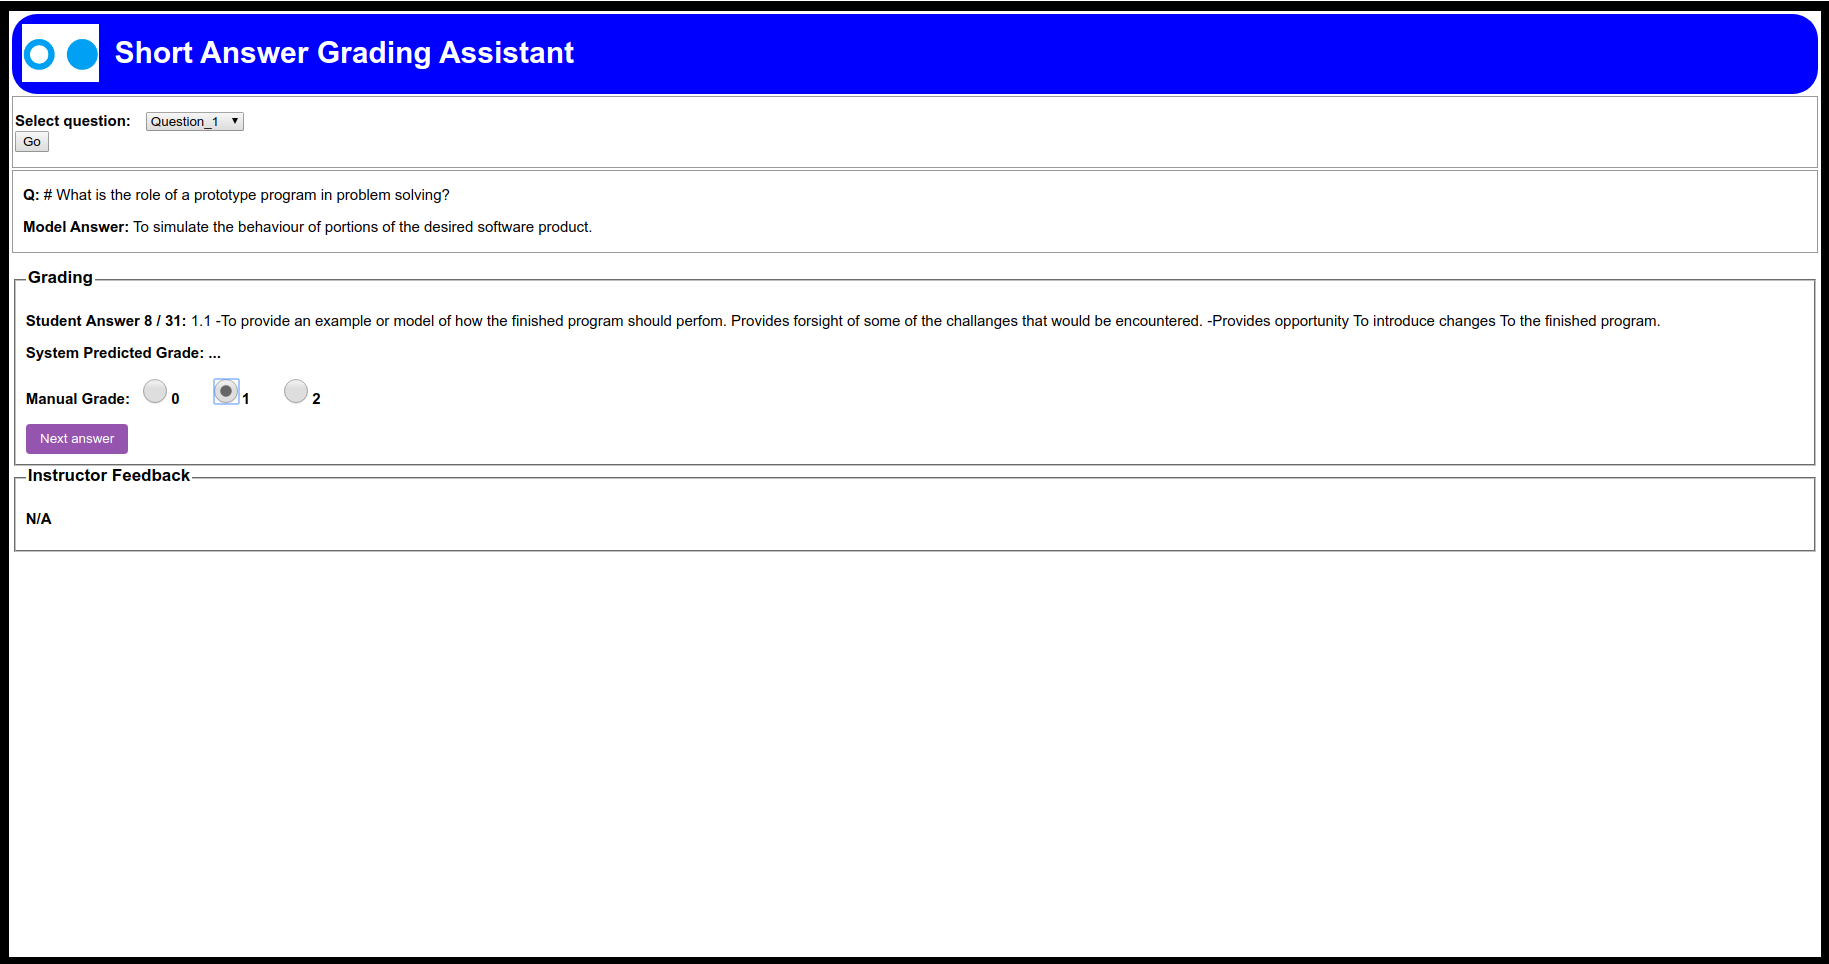
\includegraphics[width=0.48\textwidth, height=0.3\textwidth]{images/gui2.png}}
\caption{GUI display during the initial annotation stage.}
\label{fig:gui2}
\end{figure}
After a fixed set of answers are graded by the users, the tool starts assigning grades to the remaining unseen answers. Figure \ref{fig:gui3} shows the GUI display during this stage where the features contributing to the grade are highlighted in a color specific to that grade. In our implementation, a features influencing a score of 2 points are highlighted in green, those for 1 points are highlighted in yellow and red for zero points.
\begin{figure}[H]
\framebox{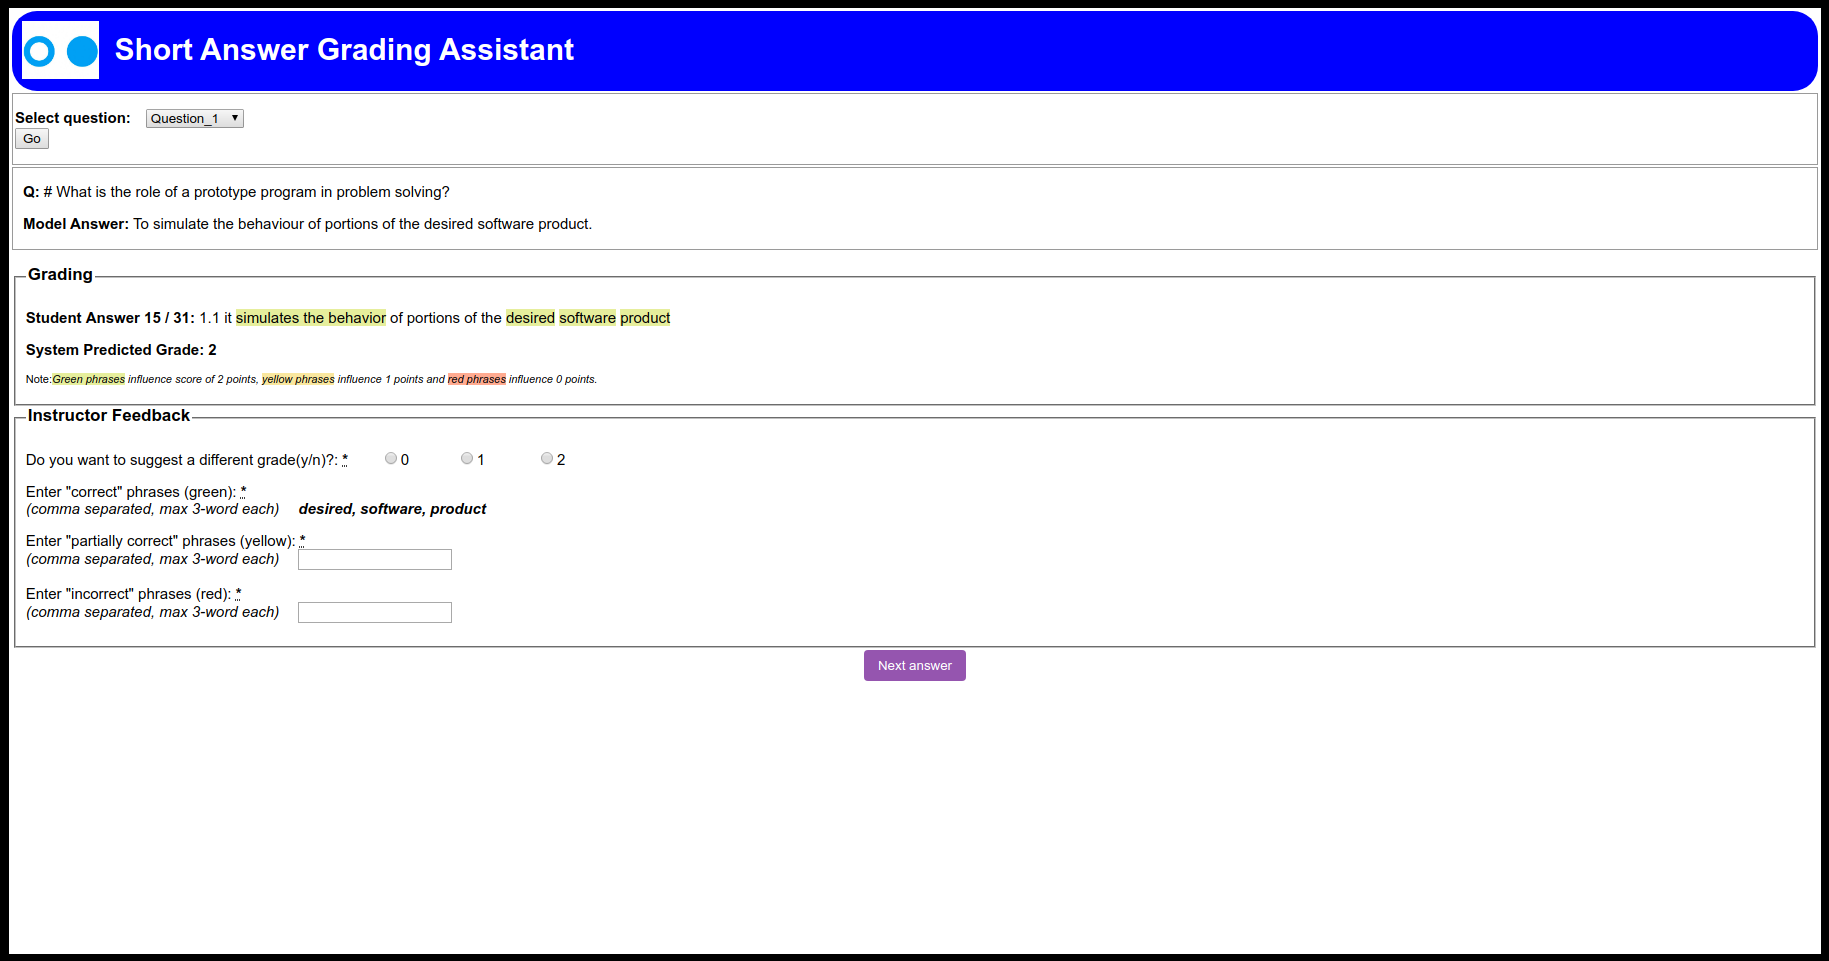
\includegraphics[width=0.48\textwidth, height=0.3\textwidth]{images/gui3.png}}
\caption{GUI display during the autograding and feedback stage.}
\label{fig:gui3}
\end{figure}
As seen in Figure \ref{fig:gui3}, phrases upto three words and not just single words are highlighted as part of the explanation. In addition, the human user may provide feedback in case of a disagreement with the system predicted grade and explanation that helps to subsequently improve the grades and explantions for the new unseen answers.\\
The results of the quantitative evaluation done by repeating the procedure carried out in our preinvestigations, i.e, using a Likert scale of 3 values (1,2 and 3) to score the degree of the acceptance of the displayed explanation for every answer to all questions from Mohler's dataset used as case studies, and then using the SciPy library’s interpolation function to map the maximally occurring score for a question into the ranges [0,0.33], [0.34,0.66] and [0.67,1] (for 1, 2 and 3 respectively) is shown in Figure \ref{fig:comparison2}.
\begin{figure}[H]
\framebox{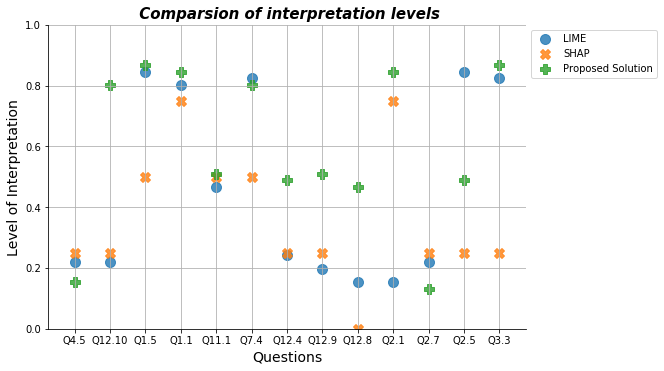
\includegraphics[width=0.48\textwidth, height=0.34\textwidth]{images/all_categ2.png}}
\caption{Quantitative Interpretation Level comparison of LIME, SHAP and the proposed solution for different questions.}
\label{fig:comparison2}
\end{figure}
We observe that in the majority of the cases, the performance from the proposed solution in terms of the level of interpretation gained from the explanation is better than or is at least as good as that obtained from LIME and SHAP.
\section{USABILITY STUDY} 
Since the development of the autograding assisting system is geared towards use in examinations and in-house assignments, a user evaluation was conducted at the University of Applied Sciences Bonn-Rhein-Sieg aimed at assessing the quality of the developed grading system through interacting with real users, and thereby determining the requirements and limitations that were overlooked due to the experimenter's bias. A full-time member of the University's lecturing staff and four other research associates were asked to attempt using the software to grade a number of questions from the Mohler's dataset as part of the evaluation study. Prior to the evaluation, each user was given a brief presentation on the usage of the system. Each user was then asked to grade multiple questions from the dataset. The questions selected differed in the length of the responses required from the students. The users were asked to `think out loud' and their words and actions were video recorded. The completion of the grading of all student answers to one question was immediately accompanied by a short online questionnaire to determine whether the explanations given was useful to the users.
\section{CONCLUSIONS}

....

\addtolength{\textheight}{-12cm}   % This command serves to balance the column lengths
                                  % on the last page of the document manually. It shortens
                                  % the textheight of the last page by a suitable amount.
                                  % This command does not take effect until the next page
                                  % so it should come on the page before the last. Make
                                  % sure that you do not shorten the textheight too much.

%%%%%%%%%%%%%%%%%%%%%%%%%%%%%%%%%%%%%%%%%%%%%%%%%%%%%%%%%%%%%%%%%%%%%%%%%%%%%%%%



%%%%%%%%%%%%%%%%%%%%%%%%%%%%%%%%%%%%%%%%%%%%%%%%%%%%%%%%%%%%%%%%%%%%%%%%%%%%%%%%



%%%%%%%%%%%%%%%%%%%%%%%%%%%%%%%%%%%%%%%%%%%%%%%%%%%%%%%%%%%%%%%%%%%%%%%%%%%%%%%%
%\section*{APPENDIX}

%....

\section*{ACKNOWLEDGMENT}

....



\begin{thebibliography}{99}

\bibitem{c1} Marco Tulio Ribeiro, Sameer Singh, and Carlos Guestrin. ``why should I trust you?": Explaining the predictions of any classifier. In Proceedings of the 22nd ACM SIGKDD International Conference on Knowledge Discovery and Data Mining, San Francisco, CA, USA, August 13-17, 2016, pages 1135-1144, 2016.
\bibitem{c2} Scott M Lundberg and Su-In Lee. A unified approach to interpreting model predictions. In Advances in Neural Information Processing Systems, pages 4765-4774, 2017.
\end{thebibliography}




\end{document}
